%======================================================================
\subsection{BW-PDM-14 --- Built, 1 Nov: simulations in the vault}\label{sec:pdm14-built}
%======================================================================

Built on your answers of 1 Nov (\S\ref{sec:pdm14-plan}), phases P1--P4 in five commits; the release phase was dropped
by your answer P6. All of it runs on a copy of your Vector vault (below); your real vault was only read.

\begin{figure}[!htbp]
\centering
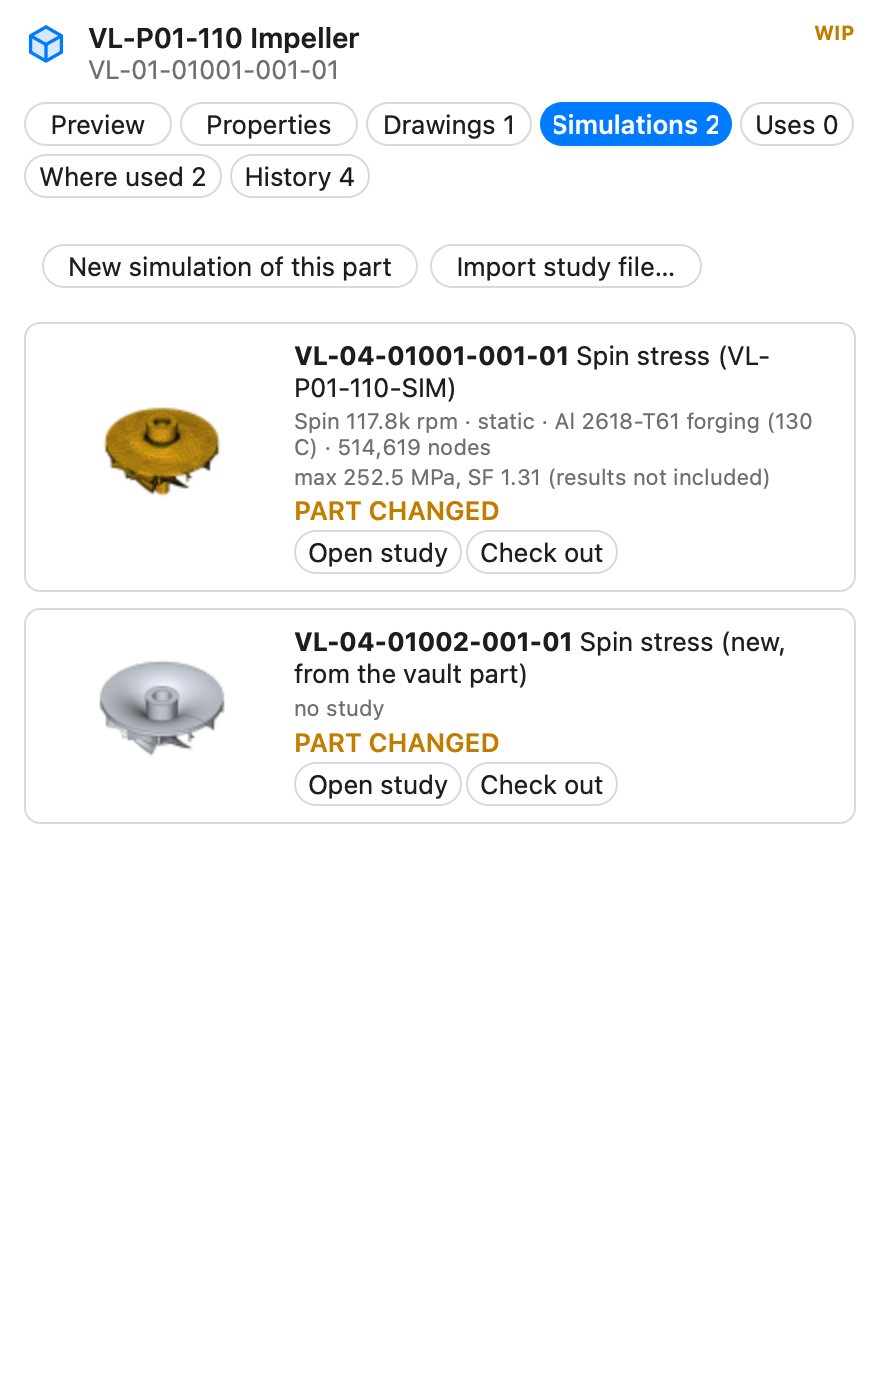
\includegraphics[width=0.36\linewidth]{fig/pdm14_simtab.png}\hfill
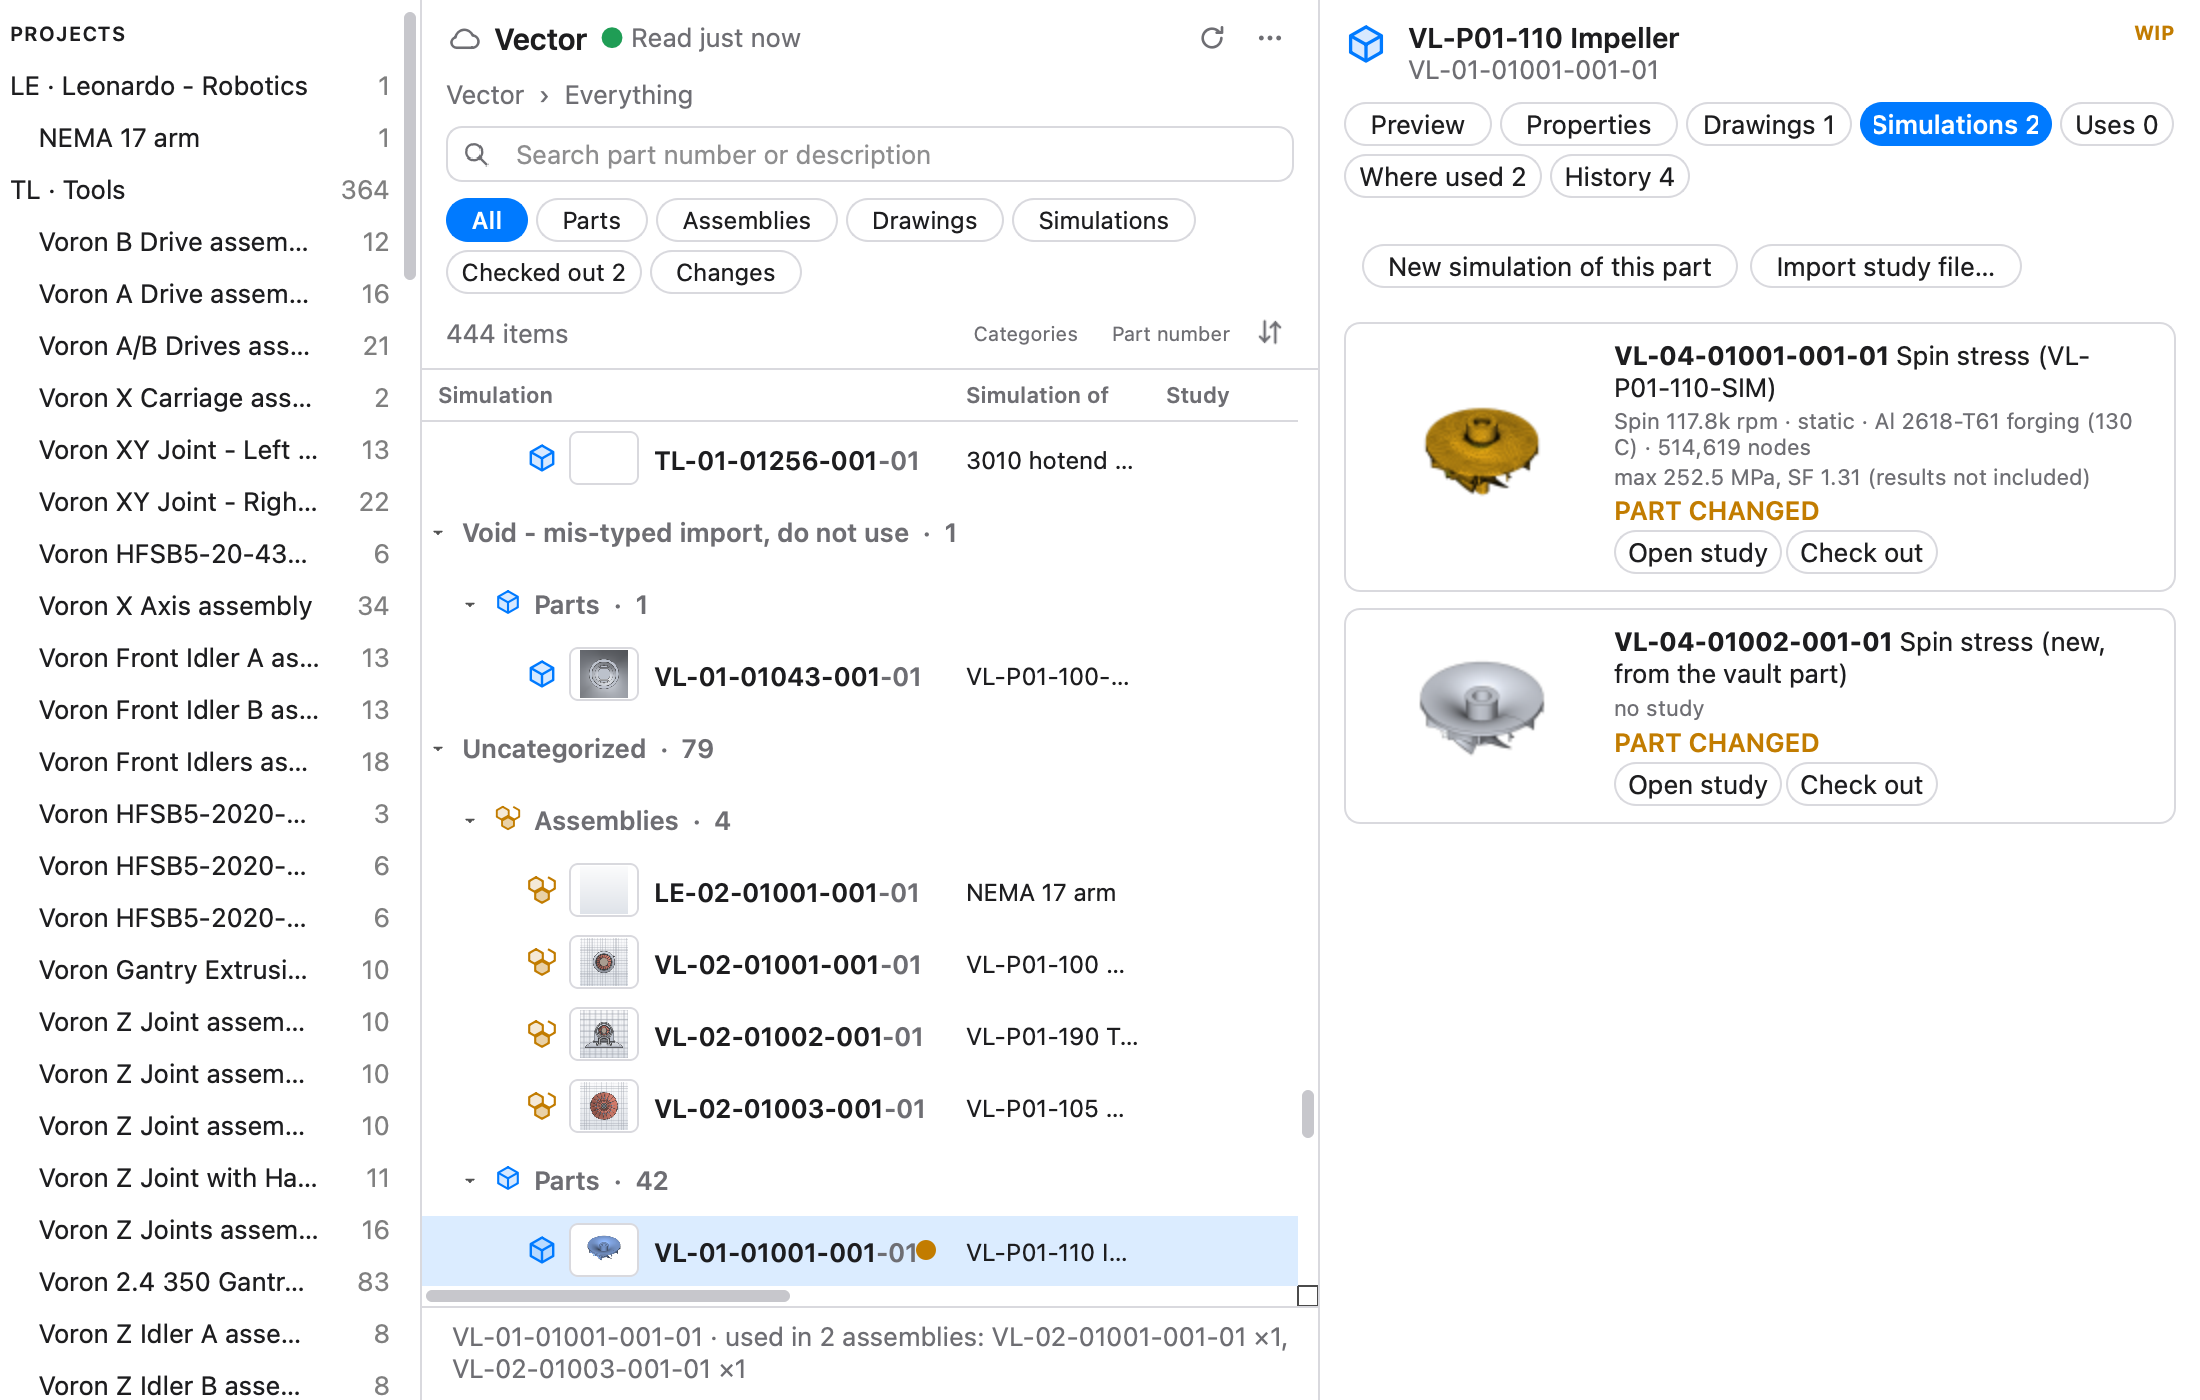
\includegraphics[width=0.60\linewidth]{fig/pdm14_files.png}
\caption{Left: the impeller's \emph{Simulations} tab on the vault copy: the imported study (picture read from inside the
file, material, 514\,619 nodes, maximum stress and safety factor, \emph{results not included}) and a new simulation made
from the vault part, both marked \emph{part changed} because the impeller was checked in with different geometry
afterwards. Right: the Files list with the \emph{Simulations} chip; the amber dot after the impeller's number is the
bubble flag.}
\label{fig:pdm14-built}
\end{figure}

\paragraph{What you can do now.}
\begin{itemize}[nosep]
  \item \textbf{A simulation is an item} (\code{simulation}, document type 04, \code{VL-04-01001-001}) with
        \code{simulation\_of} checked like \code{drawing\_of}, kept through a renumber, written to the journal only for a
        simulation, so older journals read as before. A vault made before this gets type 04 added at the first
        simulation. Storing a version now streams the file in 1\,MB blocks.
  \item \textbf{The \file{.vlsim} file.} A FreeCAD document zip with another name. File $>$ Open, Open Recent, the Start
        page and Finder open it with Heuretes FreeCAD; Save and Save As keep the extension; the vault stores and fetches it like
        an \file{.FCStd}; the picture and mesh are read from inside it.
  \item \textbf{A summary inside the file}, rewritten at every save: study type, solver, material, mesh nodes, elements and
        order, maximum von Mises, maximum displacement, minimum safety factor, bore and burst numbers, the pre-check verdict,
        solved-at, and the geometric fingerprint of the study's solid and of the part version it was copied from. The part's
        file gets its fingerprint at every save and at check-in. \emph{Current} = equal fingerprints, otherwise
        \emph{part changed}, \emph{unknown} when either side has none yet.
  \item \textbf{Include results} at check-in (remembered). Unticked, the version has no result objects and no result
        meshes; the study, solid copy, mesh settings and summary stay, the summary keeps its numbers and says so. Your work
        copy becomes that smaller copy and the file with results is kept in the work folder's \file{.results}. The item's
        history says \emph{with results} or \emph{no results} per version.
  \item \textbf{Show them}: a \emph{Simulations} chip (Simulation, Simulation of, Study, Result, Geometry), the part's
        \emph{Simulations} tab with a card per simulation (\emph{Open study}, \emph{Check out}, \emph{Report PDF} when a
        \code{<P/N>\_*\_report.pdf} is in your work folder), the bubble flag on the part's row with a tooltip, the view
        \emph{Simulation out of date}. Nothing opens a \file{.vlsim} to list it: the entries are read from the zip directory,
        cached by the version's hash (through \code{canonical()} after PRF-04), and a file still in iCloud is not downloaded.
  \item \textbf{New simulation of this part} (tab button) numbers the item, copies the solid into a new \file{.vlsim} and checks
        it out; \textbf{Import study file} brings in an existing study by naming its part. For the project pages:
        \code{vault\_trees.simulations(structure, scope)} (API note in the agents' folder).
\end{itemize}

\paragraph{Why \file{.vlsim} is only a door.} \code{FreeCAD.openDocument} never looks at the extension, so the format needed
no new code: an import type for \file{*.vlsim} (File $>$ Open, Open Recent, command line), one condition in
\code{Document::saveAs} so Save As keeps the extension, the bundle's \code{CFBundleDocumentTypes} and the
\code{QFileOpenEvent} for Finder. A converter or a document subclass would have cost a second copy of the zip code.

\paragraph{Acceptance, on a copy of the Vector vault} (442 items, 114 files migrated by PRF-04 already):
\begin{itemize}[nosep]
  \item The impeller (\code{VL-01-01001-001}) was checked in once: fingerprint \code{f03a19c8612e} (volume 17\,330.2\,mm$^3$,
        area 15\,618.9, 494 faces) written into the file and found by the card.
  \item \code{VL-P01-110-SIM.FCStd} (149\,033\,495 bytes, a copy) imported as \code{VL-04-01001-001}: 40--55\,s (it is opened,
        given its summary and saved once), checked in with results: 149.8\,MB. Its card, built without fetching the file
        (\code{fetch} was made to raise), took 1\,ms: ``max 252.5\,MPa, SF 1.31'', 514\,619 nodes, Al 2618-T61.
  \item Checked in again \emph{without results}: 33.4\,MB (the 514\,619-node mesh stays, the results go); the card reads
        ``max 252.5\,MPa, SF 1.31 (results not included)''; the history lists v1 with and v2 without results.
  \item The imported study is \emph{part changed} from the start, honestly: its solid has volume 30\,922.7\,mm$^3$ and 117 faces,
        the vault's impeller 17\,330.2 and 494. They are two different models of the impeller (the study came from the Vector Jet
        session's script). A simulation made \emph{from the vault part} (\code{VL-04-01002-001}, 1.3\,MB, 1.1\,s) is \emph{current}.
  \item The impeller was then checked in moved by 0.5\,mm (fingerprint \code{c42187a069aa}): both simulations became
        \emph{part changed} and the part got the bubble flag.
\end{itemize}

\paragraph{Decided while building.}
\begin{itemize}[nosep]
  \item The study's solid is the preview mesh of a simulation (a study hides its solid under the result).
  \item FreeCAD drops zip entries it does not know at every save, so the summary is rewritten after each save from the document;
        its previous copy (solved-at, the numbers of a copy saved without results) is read just before the save.
  \item The fingerprint is the SIM-07 one, \code{H(``geo'', geometry\_settings(shape))}; the part's shape is the first model
        candidate of its document, so a part with several visible bodies is judged by the first one.
  \item A part checked in before PDM-14 has no fingerprint: its simulations read \emph{unknown} until it is saved or checked in
        once more.
  \item The GUI test runs crash with \code{QT\_QPA\_PLATFORM=offscreen} (the main window creates a QOpenGLWidget), so they ran
        on the normal display with the window placed on the right half.
\end{itemize}

\paragraph{Tests.} Add-on suite 716 tests pass (20 new in \file{test\_vault\_simulations.py}); GUI: TestBruceWorxVlsim (2),
TestBruceWorxSimVault (4: copy and fingerprints agree, summary after save, a solved cantilever then a copy without results),
TestBruceWorxVaultBrowser (16, 4 new), VaultClient (40), Preview (12), Start (34).

\paragraph{Open questions.}
\begin{itemize}[nosep]
  \item Replace the vault's impeller with the model the study was made from, or re-copy the study from the vault impeller?
        They differ by almost a factor of two in volume.
  \item The stripped copy keeps the 514\,619-node mesh (33\,MB). Drop the mesh too for drafts, and re-mesh on open?
  \item Save As in the file dialog still lists only \file{*.FCStd}; typing a \file{.vlsim} name works. Add the filter?
\end{itemize}
